Usando la ecuación de diferencia, construir un sistema lineal para las distribuciones de calor en los siguientes puntos interior de la placa calentada cuyos temperaturas al borde se mantienen constantes.

\begin{center}
    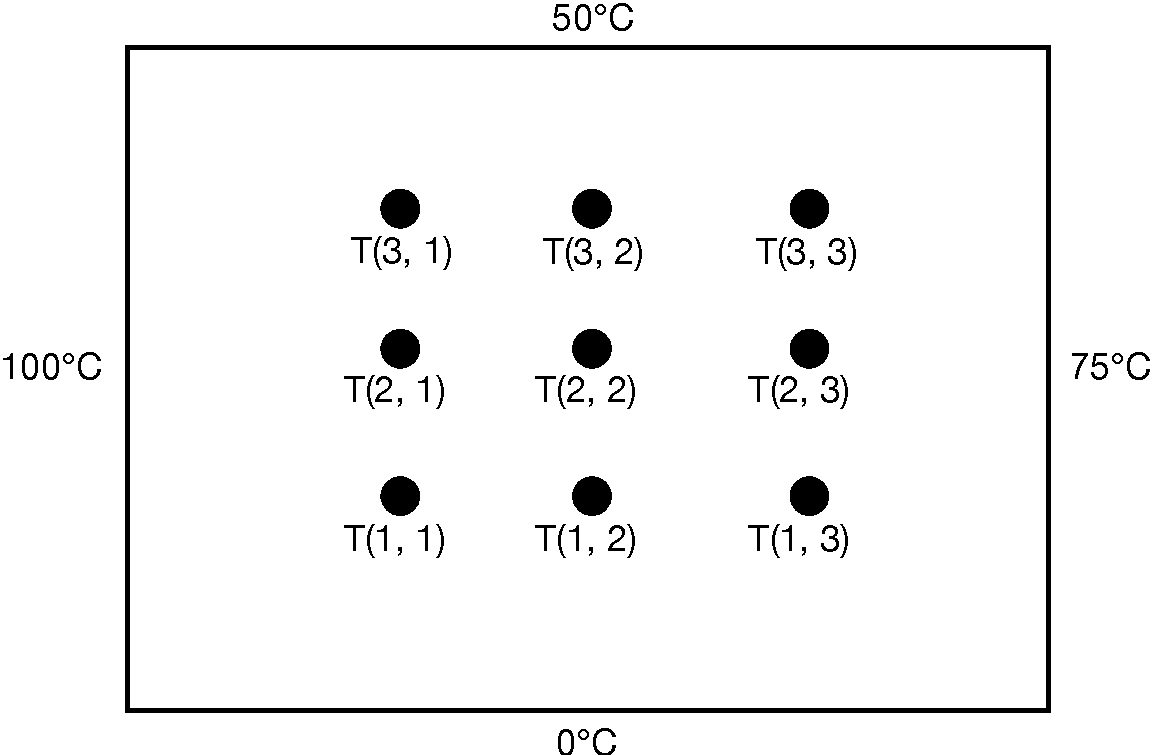
\includegraphics[scale=0.5]{images/heatingmap.pdf}    
\end{center}

Para la discretización de la placa usaremos un \textit{stencil} para generar el sistema:

\begin{center}
    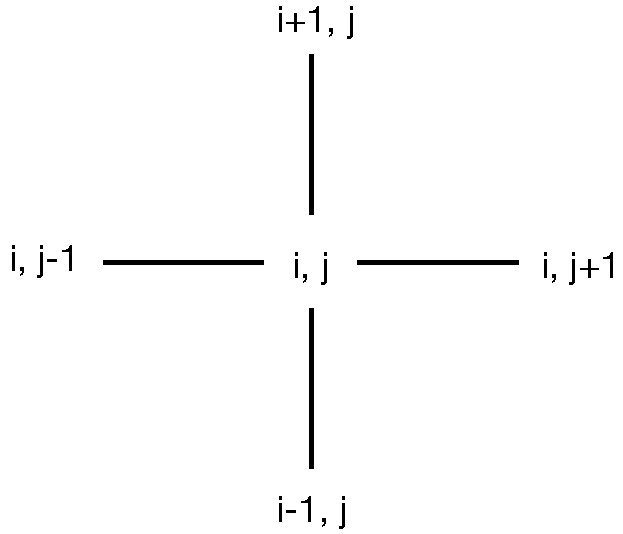
\includegraphics[scale=0.5]{images/stencil.pdf}
\end{center}

La ecuación en diferencias que describe éste \textit{stencil} (discretización de la ecuación elíptica) es la siguiente:

\begin{align}
    \frac{T_{i,j+1} + T_{i,j-1} + T_{i+1,j} + T_{i-1,j} - 4 \times T_{i, j}}{h^2} = 0
\end{align}

Usando éste \textit{stencil}, tendremos que al aplicarlo sobre la grilla $3 \times 3$ en la cual se ha discretizado la placa tendremos las siguientes 9 ecuaciones:

\begin{align*}
T_{1,2} + T_{1,0} + T_{2,1} + T_{0,1} - 4 \times T_{1, 1} &= 0\\
T_{1,3} + T_{1,1} + T_{2,2} + T_{0,2} - 4 \times T_{1, 2} &= 0\\
T_{1,4} + T_{1,2} + T_{2,3} + T_{0,3} - 4 \times T_{1, 3} &= 0\\
T_{2,2} + T_{2,0} + T_{3,1} + T_{1,1} - 4 \times T_{2, 1} &= 0\\
T_{2,3} + T_{2,1} + T_{3,2} + T_{1,2} - 4 \times T_{2, 2} &= 0\\
T_{2,4} + T_{2,2} + T_{3,3} + T_{1,3} - 4 \times T_{2, 3} &= 0\\
T_{3,2} + T_{3,0} + T_{4,1} + T_{2,1} - 4 \times T_{3, 1} &= 0\\
T_{3,3} + T_{3,1} + T_{4,2} + T_{2,2} - 4 \times T_{3, 2} &= 0\\
T_{3,4} + T_{3,2} + T_{4,3} + T_{2,3} - 4 \times T_{3, 3} &= 0\\
\end{align*}

Aplicando las condiciones de borde, podemos reducir el sistema al siguiente:

\begin{align*}
T_{1,2} + T_{2,1} - 4 \times T_{1, 1} &= - T_{1,0} - T_{0,1} = -0 - 100 = -100\\
T_{1,3} + T_{1,1} + T_{2,2} - 4 \times T_{1, 2} &= -T_{0,2} = -0 = 0\\
T_{1,2} + T_{2,3} - 4 \times T_{1, 3} &= 0 = -T_{1,4} - T_{0,3} = -75 - 0 = -75 \\
T_{2,2} + T_{3,1} + T_{1,1} - 4 \times T_{2, 1} &= -T_{2,0} = -100 \\
T_{2,3} + T_{2,1} + T_{3,2} + T_{1,2} - 4 \times T_{2, 2} &= 0\\
T_{2,2} + T_{3,3} + T_{1,3} - 4 \times T_{2, 3} &= -T_{2,4} = -75\\
T_{3,2} + T_{2,1} - 4 \times T_{3, 1} &= -T_{3,0} - T_{4,1} = -100 -50 = -150\\
T_{3,3} + T_{3,1} + T_{2,2} - 4 \times T_{3, 2} &= -T_{4,2} = -50\\
T_{3,2} + T_{2,3} - 4 \times T_{3, 3} &= -T_{3,4} - T_{4,3} = -75 - 50 = -125\\
\end{align*}

La cual genera el siguiente sistema:

\[
    \begin{bmatrix}
        -4 & 1 & 0 & 1 & 0 & 0 & 0 & 0 & 0 \\
        1 & -4 & 1 & 0 & 1 & 0 & 0 & 0 & 0 \\
        0 & 1 & -4 & 1 & 0 & 1 & 0 & 0 & 0 \\
        1 & 0 & 1 & -4 & 1 & 0 & 1 & 0 & 0 \\
        0 & 1 & 0 & 1 & -4 & 1 & 0 & 1 & 0 \\
        0 & 0 & 1 & 0 & 1 & -4 & 1 & 0 & 1 \\
        0 & 0 & 0 & 1 & 0 & 1 & -4 & 1 & 0 \\
        0 & 0 & 0 & 0 & 1 & 0 & 1 & -4 & 1 \\
        0 & 0 & 0 & 0 & 0 & 1 & 0 & 1 & -4 \\
    \end{bmatrix}
\]